\documentclass[a4paper,11pt]{kth-mag}
\usepackage[T1]{fontenc}
\usepackage{textcomp}
\usepackage{lmodern}
\usepackage[utf8]{inputenc}
\usepackage{csquotes}
\usepackage[swedish,english]{babel}
\usepackage{modifications}
\usepackage[backend=biber]{biblatex}
\usepackage{hyperref}
\hypersetup{
}
\usepackage{listings}
\usepackage{tikz}
\usetikzlibrary{arrows,positioning}
\usepackage{todonotes}

\lstset{%
  frame=L,
  basicstyle=\tiny,
  xleftmargin=\parindent
}

\bibliography{bibliography.bib}

\newcommand{\code}[1]{\texttt{#1}}

\newenvironment{metatext}{%
  \textbf{$\hookrightarrow$}
  \begin{itshape}
}{
  \end{itshape}
  \newline
  \newline
  \useignorespacesandallpars
}

\def\useignorespacesandallpars#1\ignorespaces\fi{%
#1\fi\ignorespacesandallpars}

\makeatletter
\def\ignorespacesandallpars{%
  \@ifnextchar\par
    {\expandafter\ignorespacesandallpars\@gobble}%
    {}%
}
\makeatother

\title{Modular responsive web design}
\foreigntitle{Modulär responsiv webbutveckling}
\subtitle{Allowing responsive web modules to respond to custom criterias instead of only viewport size by implementing \emph{element queries}}
\author{Lucas Wiener \\ \lowercase{lwiener@kth.se}}
\date{February 2015}
\blurb{Master's Thesis at \textsc{csc}\\\hfill\\ Supervisors at \textsc{evry ab}: Tomas Ekholm \& Stefan Sennerö\\Supervisor at \textsc{csc}: Philipp Haller\\Examiner: Mads Dam}
\trita{TRITA xxx yyyy-nn}
\begin{document}
  \frontmatter
  \pagestyle{empty}
  \removepagenumbers
  \maketitle
  \selectlanguage{english}
  \begin{abstract}
    Abstract goes here.
  \end{abstract}
  \clearpage
  \begin{foreignabstract}{swedish}
    Sammanfattning ska vara här.
  \end{foreignabstract}
  \clearpage
  \tableofcontents*
  \listoftodos
  \mainmatter
  \pagestyle{newchap}
  \chapter{Introduction}
    \todo{Write somewhere that modular and responsive web development right now is two disjunct terms?}
    \todo{This or the thesis? Now both is being used.}
    \todo{runtime or run time? same for parse time. Both is being used right now.}
    \todo{Container or parent element? Using both now.}
    \section{Targeted audience}
      The thesis is targeted for web developers that wish to gain a deeper understanding of element queries and how one could solve the problem today.
      Heavy use of web terminology is being used and intermediate web development knowledge is assumed.
    \section{Problem statement}
      By using \textsc{css} \emph{media queries} developers can specify different style rules for different viewport sizes.
      This is fundamental to creating responsive web applications.
      If developers want to build modular applications by composing the application by smaller components (elements, scripts, styles, etc.) media queries are no longer applicable.
      Modular responsive components should be able to react and change style depending on the size that the component has been given by the application, not the viewport size.
      The problem can be formulated as: \emph{Elements can not specify conditional style rules depending on their own size, or the size of any other element}.
      See the included document in section~\ref{sec:problem-formulation} of the appendix for a more practical problem formulation.

      \todo{Back this up or maybe reformulate it a bit.}
      The main international standards organization for the World Wide Web (World Wide Web Consortium, abbreviated \textsc{w3c}) has unofficially stated that such feature would be infeasible to implement.
      Some problems with implementing element queries in \textsc{css} are:
      \begin{itemize}
        \item \textbf{Circularity:}
        If style rules can be applied by criterias of other elements, it will be possible to create cyclic rules (infinite loops of styling).
        Some cyclic rules might be possible to detect during \textsc{css} parsing, but there are so many combinations of style properties that could result in cyclic rules that it will add a lot of complexity to the language, both for implementers and users.
        Also, it has been shown that some cyclic rules are impossible to detect at parse time, due to being dependent on run time factors.
        See section~\ref{sec:cyclic-rules} for examples and a deeper analysis of cyclic rules.
        \item \textbf{Performance:} 
        \todo{Rewrite this. Some of this is totally wrong.}
        layout engines typically perform selector matching and layout computations in parallel to achieve good performance.
        If element queries would be implemented, the layout engines would need to first compute the layout of all elements in order to decide which selectors would conform to the element query conditions and then do a new layout computation, and so on until a stable state has been reached.
        Far worse, since selectors now depend on layout style, this cannot be done in parallel which impacts performance heavily.
      \end{itemize}
      \todo{Back this up or rewrite.}
      Because of the problems, it is stated that such feature will not be implemented in the near future. So it is now up to the developers to implement this feature as a third-party solution.
      Efforts have been made to create a robust implementation, with moderate success.
      Since all implementations have shortcomings, there is still no de facto solution that developers use and the problem remains unsolved.

    \section{Objective}
      The main objective of this thesis is to develop a third-party implementation of element queries (or equivalent to solve the problem of modular responsive components).
      To do this, it is needed to research existing implementation attempts in order to understand and analyze the advantages and shortcomings of the approaches.
      It is also neccesary to be aware of the premises, such as browser limitations and specifications that need to be conformed.
      In addition, research will be done about the problems of implementing element queries natively, to get a deeper understanding of how an official \textsc{api} would look like.
      There are many challenges along the way that will need to be researched and worked around.
      Examples of such subproblems that would need to be investigated are:
      \begin{itemize}
        \item How should circularity be handled? Should it be detected at runtime or parsetime, and what should happen on detection?
        \item How can one listen to element size changes without any native support?
        \item How can a custom \textsc{api} be crafted that will enable element queries and still conform to the \textsc{css} specification?
        \item If a custom \textsc{api} is developed, how would one make third-party modules (that uses media queries) work without demanding a rewrite of all third-party modules?
      \end{itemize}
      The scientific question to be answered is if it is possible to solve the problem  without extending the current web standard.
      The hypothesis is that the problem can be solved in a reliable and performant way by crafting a third-party implementation.
      \todo{This might be a bit to much.}
      A reliable implementation should also enable existing responsive components to react to a specified criteria (parent container size for example) with no modifications to the components.
      The goal of the thesis should be considered fulfilled if a solution was successfully implemented or described, or if the problems hindering a solution are thoroughly documented.

    \section{Significance}
      Many frameworks and techniques are being used in web development to keep the code from becoming an entangled mess.
      Creating modules helps to ease development and increase reusability.
      One of the biggest issues that keeps web modules from being truly modular is that they cannot adapt to given sizes.
      This makes the modules either force the client to style them properly depending on viewport size, or not being responsive.
      Both options are undesirable for developing larger applications.
      A third option would be to make the modules context aware and style themselves according to the viewport, which defeats the purpose of modules (making them not reusable).

      The last couple of years a lot of articles have been written about the problem and how badly we need element queries.
      As already stated, third-party implementation efforts have been made by small and big players, with moderate success.
      \textsc{w3c} keep getting requests and questions about it, but the answer seems to lean towards no.
      An organization called Responsive Issues Community Group (abbreviated \textsc{ricg}) have started an initial planning regarding element queries.
      However, things are moving slow and a draft about element queries use cases are still being made.

      Solving this problem would be a big advancement to web development, enabling developers to create truly modular components.
      By studying the problem, identifying approaches and providing a third-party solution the community can take a step closer to solve the problem.
      If the hypothesis holds, developers will be able to use element queries in the near future, while waiting for \textsc{w3c} to make their verdict.
      The outcome of this thesis can also be helpful for \textsc{w3c} and others to get an overview of the problem and possibly get ideas how subproblems can be handled.
    \section{Methodology}
      \todo{What should go here?}
    \section{Delimitations}
      The focus of the thesis lays on developing a third-party framework that realizes element queries.
      All theoretical studies and work will be performed to support the development of the framework.

      \subsection{What will be done}
      \begin{itemize}
      \item A third-party implementation of element queries will be developed.
      \item The problems of implementing element queries natively will be addressed.
      \item Theory about layout engines, \textsc{css}, \textsc{html} and responsive web design will be given to fully understand the problem.
      \end{itemize}

      \subsection{What will not be done}
      \begin{itemize}
      \item No efforts will be made to solve the problems accompanied with a native solution.
      \item No \textsc{api} or similar will be designed for a native solution.
      \item \textsc{ui} and \textsc{ux} design will not be addressed, other than necessary for understanding the problem.
      \item No complete history of browsers, the Internet or responsive web design will be given other than neccesary.
      \end{itemize}
    \section{Outline}

  \part{Background}

    \chapter{Browsers} 
      \begin{metatext}
        Browsers and the Internet is something that many people today take for granted.
        It is not longer the case that only computer scientists are browsing the web.
        Today the web is becoming increasingly important in both our personal and professional lives.
        This chapter will give a brief history of browsers and the rise of the web.
        This section is a summary of \normalfont{\cite{internet_live_stats}\cite{internet_of_things}\cite{wiki_hypermedia}\cite{w3c_www}\cite{oed}}.
      \end{metatext}

      Before addressing the birth of the web, lets define the meaning of the concepets of the \emph{Internet}, \emph{Web} and \emph{World Wide Web}.
      The word internet can be translated to \emph{something between networks}. 
      When referring to the Internet (capitalized) it is usually the global decentralized internet used for communication between millions of networks using \textsc{tcp/ip}.
      Since the Internet is decentralized, there is no owner.
      Or in other words, the owners are all the network end-points which means all users of the Internet.
      One can argue that the owners of the Internet are the \textsc{isp}'s, providing the services and infrastructure making the Internet possible.
      On the other hand, the backbones of the Internet are usually co-founded by countries and companies.
      Or is it the \textsc{icann}\footnote{The Internet Corporation for Assigned Names and Numbers} organization which has the responsibility for managing the \textsc{ip} addresses in the Internet namespace?
      Clearly, the Internet wouldn't be what it is today without all the actors.
      The Internet lays the ground for many systems and applications, including the World Wide Web, file sharing and telephony.
      In 2014 the number of Internet users was measured to just below 3 billions, and estimations shows that we have surpassed 3 billions users today (no report for 2015 has been made yet).
      Users are here defined as humans having unrestricted acccess to the Internet.
      If one instead measures the number of connected entities (electronic devices that communicates through the Internet) the numbers are much higher.
      An estimation for 2015 of 25 billions connected entities has been made, and the estimation for 2020 is 50 billions.
      
      As already stated, the Word Wide Web (abbreviated \textsc{www} or \textsc{w3}) is a system that operates through the Internet.
      The World Wide Web is usually shortened to simply \emph{the web}.
      The web is a system for accessing interlinked hypertext documents and other media such as images and videos.
      Since not only hypertext is interlinked on the web, the term \emph{hypermedia} can be used as an extension to hypertext which also includes other nonlinear medium of information (images, videos, etc.).
      Although the term hypermedia has been around for a long time, the term hypertext is still being used as synonym for hypermedia.
      Further, the web can also be referred to as the universe of information accessible through the web system.
      Therefore, the web is both the system enabling sharing of hypermedia and also all of the accessible hypermedia itself.
      Hypertext documents are today more known by the name \emph{web pages} or simply \emph{pages}.
      Multiple related pages compose a \emph{web site} or simply a \emph{site} and are usually hosted from the same domain.
      To transfer the resources between computers the protocol \textsc{http} is used.
      Typically the way of retrieving resources on the web is by using a \emph{web browser} or simply a \emph{browser}.
      Browsers handles the fetching, parsing and rendering of the hypertext (more about this in section~\ref{sec:browsers}).
      
      \section{The origin of the web}
        \begin{metatext}
          Since the web is a system operating on top of the Internet, it is needed to first investigate the origin of the Internet.
          This can be viewed from many angles and different aspects need to be taken into consideration.
          With that in mind, the origin of the Internet is not something easily pinned down and what will be presented here will be more of a technically interesting history.
          This section is a summary of \normalfont{\cite{overview_of_tcp_ip}\cite{internetsociety_history_internet}\cite{internet_maps}\cite{historyofthings_internet}}.
        \end{metatext}

        In the early 1960's \emph{packet switching} was being researched, which is a prerequisite of internetworking.
        With packet switching in place, the very important ancestor of the Internet \textsc{arpanet} (Advanced Research Projects Agency Network) was developed, which was the first network to implement the \textsc{tcp/ip} protocol suite.
        The \textsc{tcp/ip} protocol suite together with packet switching are fundamental technologies of the Internet.
        \textsc{arpanet} was funded by the United States Department of Defense (DoD) in order to interconnect their research sites in the United States.
        The first nodes of \textsc{arpanet} was installed at four major universities in the western United States in 1969 and two years later the network spanned the whole country.
        The first public demonstration of \textsc{arpanet} was held at the International Computer Communication Conference (ICCC) in 1972.
        It was also at this time the email system was introduced, which became the largest network application for over a decade.
        In 1973 the network had international connections to Norway and London via a sattelite link.
        At this time information was exchanged with the File Transfer Protocol (\textsc{ftp}), which is a protocol to transfer files between hosts.
        This can be viewed as the first generation of the Internet. With around 40 nodes, operating with raw file transfers between the hosts it was mostly used by the academic community of the United States.

        The number of nodes and hosts of \textsc{arpanet} increased slowly, mainly due to the fact that it was a centralized network owned and operated by the \textsc{us} military.
        In 1974 the \textsc{tcp/ip} stack was proposed in order to have a more robust and scalable system for end-to-end network communication.
        The \textsc{tcp/ip} stack is a key technology for the decentralization of the \textsc{arpanet}, to allow the massive expandation of the network that later happened.
        In 1983 \textsc{arpanet} switched to the \textsc{tcp/ip} protocols, and the network was split in two.
        One network was still called \textsc{arpanet} and was to be used for research and development sites.
        The other network was called \textsc{milnet} and was used for military purposes.
        The decentralization event was a key point and perhaps the birth of the Internet.
        The Computer Science Network (\textsc{csnet}) was funded by the National Science Foundation (\textsc{nsf}) in 1981 to allow networking benefits to academic insitutions that could not directly connect to \textsc{arpanet}.
        After the event of decentralizing \textsc{arpanet}, the two networks were connected among many other networks.
        In 1985 \textsc{nsf} started the National Science Foundation Network (nsfnet) program to promote advanced research and education networking in the \textsc{us}.
        To link the supercomputing centers funded by \textsc{nsf} the \textsc{nsfnet} serverd as a high speed and long distance backbone network.
        As more networks and sites were linked by the \textsc{nsfnet} network, it became the first backbone of the Internet.
        In 1992, around 6000 networks were connected to the \textsc{nsfnet} backbone with many international networks.
        To this point, the Internet was still a network for scientists, academic institutions and technology enthusiasts.
        Mainly, because \textsc{nsf} had stated that \textsc{nsfnet} was a network for non-commercial traffic only.
        In 1993 \textsc{nsf} decided to go back to funding research in supercomputing and high-speed communcations instead of funding and running the Internet backbone.
        That, along with an increasing preassure of commercializing the Internet let to another key event in the history of the Internet - the privatization of the \textsc{nsfnet} backbone.

        In 1994, the \textsc{nsfnet} was systematically privatized while making sure that no actor owned too much of the backbone in order to create constructive market competition.
        With the Internet decentralized and privatized regular people started using it as well as companies.
        Backbones were built across the globe, more international actors and organizations appeared and eventually the Internet as we know it today came to exist.

        \subsection{The World Wide Web}\label{sec:www}
          \begin{metatext}
            Now that the history of the Internet has been described, it is time to talk about the birth of the World Wide Web.
            Here the initial ideas of the web will be described, the alternatives and how it became a global standard.
            This subsection is a summary of \normalfont{\cite{wiki_gopher}\cite{wiki_www}\cite{webdevnotes_history_of_the_internet}\cite{webdevnotes_www_basics}\cite{historyofthings_internet}}.
          \end{metatext}

          \todo{Should have another subsection or not have this in a subsection. Only one subsection is not nice.}

          Recall that the way of exchanging information was to upload and download files between clients and hosts with \textsc{ftp}.
          If a document downloaded was referring to another document, the user had to manually find the server that hosted the other document and download it manually.
          This was a poor way of digesting information and documents that linked to other resources.
          In 1989 a proposal for a communication system that allowed interlinked documents was submitted to the management at \textsc{cern}.
          The idea was to allow links embedded in text documents, to enable users to view the linked document by clicking it.
          A quote from the draft:
          \begin{quote}
            Imagine, then, the references in this document all being associated with the network address of the thing to which they referred, so that while reading this document you could skip to them with a click of the mouse.
          \end{quote}
          This catches the whole essence of the web in a sentence --- to interlink resources in an user friendly way.
          The proposal describes that such text embedded links would be hypertext.
          It continues to explain that interlinked resources does not need to be limited to text documents, multimedia such as images and videos can also be interlinked which would similarly be hypermedia.
          The concept of browsers is described, with a client-server model the browser would fetch the hypertext documents, parse them and handle the fetching of all media linked in the hypertext.

          In 1990, the Hypertext Transfer Protocol (\textsc{http}), the Hypertext Markup Language (\textsc{html}), a browser and a web server had been created and the web was born.
          One year later the web was introduced to the public and in 1993 over five hundred international web servers existed.
          It was stated in 1994 that the web was to be free without any patents or royalties.
          At this time the Wolrd Wide Web Consortium (\textsc{w3c}) was founded by Berners-Lee with support from the Defense Advanced Research Projects Agency and the European Commission.
          The organization comprised of companies and individuals that wanted to standardize and improve the web.

          As a side note, the Gopher protocol was developed in parallel to the World Wide Web by the University of Minnesota.
          It was released in 1991 and quickly gained traction as the web still was in very early stages.
          The goal of the system, just like the web, was to overcome the shortcomings of browsing documents with \textsc{ftp}.
          Gopher enabled servers to list the documents present, and also to link to documents on other servers.
          This created a strong hierarchy between the documents.
          The listed documents of a server could then be presented as hypertext menus to the client (much like a web browser).
          As the protocol was simpled than \textsc{http} it was often preferred since it used less network resources.
          The structure provided by Gopher provided a platform for large electronic library connections.
          A big difference between the web and the Gopher platform is that the Gopher platform provided hypertext menus presented as a file system while the web hypertext links inside hypertext documents, which provided greater flexibility.
          When the University of Minnesota announced that it would charge lincensing fees for the implementation, users were somewhat scared away.
          As the web matured, being a more flexible system with more features as well as being totally free it quickly became dominant.

      \section{The history of browsers}
        \label{sec:browsers}
        \begin{metatext}
          In the mid 1990's the usage of the Internet transitioned from downloading files with \textsc{ftp} to instead access resources with the \textsc{http} protocol.
          To fulfill the vision that users would be able to skip to the linked documents ``with a click of the mouse'' the users needed a client to handle the fetching and displaying of the hypertext documents, hence the need for browsers were apparent.
          Here the evolution of the browser clients will be given, while emphasizing the timeline of the popular browsers we use today.
          This section is a summary of \normalfont{\cite{wiki_www}\cite{wiki_nexus}\cite{wiki_lmb}\cite{wiki_libwww}\cite{wiki_mosaic}\cite{wiki_netscape}\cite{wiki_mozilla}\cite{wiki_opera}\cite{wiki_konqueror}\cite{wiki_safari}\cite{wiki_webkit}\cite{wiki_blink}}.
        \end{metatext}

        The first web browser ever made was created in 1990 and was called WorldWideWeb (which was renamed to Nexus to avoid confusion).
        It was at the time the only way to view the web, and the browser only worked on NeXT computers.
        Built with the NeXT framework, it was quite sophisticated.
        It had a \textsc{gui} and a \textsc{wysiwyg}\footnote{What You See Is What You Get is a classification that ensures that text and graphics during editing appears close to the result.} hypertext document editor.
        Unfortunately it couldn't be ported to other platforms, so a new browser called \emph{Line Mode Browser} (\textsc{lmb}) were quickly developed.
        To ensure compatability with the earliest computer terminals the browser displayed text, and was operated with text input.
        Since the browser was operated in the terminal, users could log in to a remote server and use the browser via telnet.
        The code that the two browsers shared was in 1993 bundled as a library called \emph{libwww}.
        The library was licensed as \emph{public domain} to encourage the development of web browsers.
        Many browsers were develop at this time.
        The \emph{Arena} browser served as a testbed browser and authoring tool for Unix.
        The \emph{ViolaWWW} browser was the first to support embedded scriptable objects, stylesheets and tables.
        \emph{Lynx} is a text based browser that supports many protocols (including Gopher and \textsc{http}), and is the oldest browser still being used and developed.
        The list of browsers of this time can be made long.

        In 1993, the \emph{Mosaic} browser was released by the National Center for Supercomputing Applications (\textsc{ncsa}) which came to be the ancestor of many of the popular browsers in use today.
        As Lynx, Mosaic also supported many different protocols.
        Mosaic quickly became popular, mainly due to the intuitive \textsc{gui}, reliability, simple installation and Windows compatability.
        The company \emph{Spyglass, Inc.} licensed the browser from \textsc{ncsa} for producing their own browser 1994.
        Around the same time the leader of the team that developed Mosaic, Marc Andreessen, left \textsc{ncsa} to start Mosaic Communications Corporation.
        The company released their own browser named \emph{Mosaic Netscape} in 1994, which later was to be called \emph{Netscape Navigator} which was internally codenamed \emph{Mozilla}.
        Microsoft licensed the Spyglass Mosaic browser in 1995, modified and renamed it to \emph{Internet Explorer}.
        In 1997 Microsoft started using their own \emph{Trident} layout engine for Internet Explorer.
        The norwegian telecommunications company \emph{Telenor} developed their own browser called \emph{Opera} in 1994, which was released 1996.
        Internet Explorer and Netscape Navigator were the two main browsers for many years, competing for market dominance.
        Netscape couldn't keep up with Microsoft, and was slowly losing market share.
        In 1998 Netscape started the open source Mozilla project, which made available the source code for their browser.
        Mozilla was to originally develop a suite of internet applications, but later switched focus to the \emph{Firefox} browser that had been created in 2002.
        Firefox uses the \emph{Gecko} layout engine developed by Mozilla.

        Another historically important browser is the \emph{Konqueror} browser developed by the free software community \textsc{kde}.
        The browser was released in 1998 and was bundled in the \textsc{kde} Software Compilation.
        Konqueror used the \textsc{kthml} layout engine, also developed by \textsc{kde}.
        In 2001, when \emph{Apple Inc.} decided to build their own browser to ship with \textsc{os x}, a fork called \emph{WebKit} was made of the \textsc{khtml} project.
        Apple's browser called \emph{Safari} was released in 2003.
        The WebKit form was made fully open source in 2005.
        In 2008, \emph{Google Inc.} also released a browser based on WebKit, named \emph{Google Chrome}, or shortened \emph{Chrome}.
        The majority of the source code for Chrome was open sourced as the \emph{Chromium} project.
        Google decided in 2013 create a fork of WebKit called \emph{Blink} for their browser.
        Opera Software decided in 2013 to base their new version of Opera on the Chromium project, using the Blink fork.

        \todo{Timeline image and text perhaps}


    \chapter{Web development}
      \begin{metatext}
        As the history of browsers has been presented, it is time to understand the evolution of web development.
        Browsers are the far most popular tools of accessing content on the web, which makes them very important in the modern society.
        In the dawn of the web, browsers were simply applications that fetched and displayed text with embedded links.
        Today, browsers act more like an operating system (on top of the host system), parsing and executing complex web applications.
        There even exist computers that only run a browser, which is sufficient for many users.
        This chapter will describe the transition from browsers rendering simple documents to being hosts for complex applications.
        It will also describe two key evolution points in web development --- responsive web design and modular development.
      \end{metatext}

      \todo{What to write here?}
      \section{From documents to applications}
        \begin{metatext}
          This section will describe the transition from browsers rendering simple documents to being hosts for complex applications.
          Since web development trends are not easily pinned to exact dates, this section will only present dates as guidance and should not be regarded as exact dates for the events.
          This section is a summary of \normalfont{\cite{wiki_web_dev}\cite{wiki_cgi}\cite{wiki_css}\cite{wiki_ajax}\cite{wiki_html5}\cite{book_html5}}.
        \end{metatext}

        As described in section~\ref{sec:www}, browsers initially were applications that displayed hypertext documents with the ability to fetch linked documents in an user friendly way.
        Static content were written in \textsc{html}, which could include hyperlinks to other hypertext documents or hypermedia.
        Different stylesheet languages were being developed to enable the possibility of separating content styling with the content.
        In 1996 \textsc{w3c} officially recommended the Cascading Style Sheets (\textsc{css}), which came to be the preferred way of styling web content.
        Since \textsc{html} is only a markup language it is not possible to generate dynamic content, which was sufficient at the time \textsc{html} only was used for annotating links in research documents.

        The need for generated dynamic content grew bigger, and \textsc{ncsa} created the first draft of the Common Gateway Interface (\textsc{cgi}) in 1993, which provides an interface between the web server and the systems that generate content.
        \textsc{cgi} programs are usually referred to as scripts, since many of the popular \textsc{cgi} languages are script langauges.
        To generate dynamic content on the server is sometimes referred to as \emph{serverside scriping}.
        This enabled developers to generate dynamic websites, with different content for different users for instance.
        However, when the content had been delivered to the client (browser) it was still static content.
        There is no way for the server to change the content that the client has received, unless the client requests another document.

        Around 1996, client side scripting was born.
        The term Dynamic \textsc{html} (\textsc{dhtml}) was being used as an umbrella term for a collection of technologies used together to make pages interactive and animated, where client side scripting played a big role.
        Examples of things that were being done with \textsc{dhtml} are; refreshing the pages for the user so that new content is loaded, give feedback on user input without involving the server and animating content.
        Plugins also existed during this time, which teaches the browsers how to handle and execute programs. \emph{Java applets} and \emph{Flash} are examples of this.
        The user then had to download the Java runtime or Flash runtime on the computer.
        When the runtimes are present, the browser then executed the included Java applets or Flash in the web pages by using the external runtimes.
        This enabled web developers to use ``real'' programming languages.
        The drawback of this is that users first had to download the runtimes in order to run the programs embedded in pages.
        As client side scripting matured and standardized into \emph{JavaScript}, plugins slowly decreased in popularity.
        With the increase of smart devices (such as phones, televisions, cars, game consoles, etc.) which included browsers but limited third-party runtimes, plugins quickly went extinct.
        Today, web sites rarely use plugins.

        As JavaScript and \textsc{html} supported more features, websites turned into small applications with user sessions (using cookies) and user interfaces.
        Still, parts of the applications were defined as \textsc{html} pages, fetched from the server when navigating the site.
        When \emph{XMLHttpRequest} \textsc{api} was supported in the major browsers, pages no longer needed to reload the page to fetch new content as XMLHttpRequest enabled developers to perform asynchronous requests to the server without page reload.
        This opened up for \emph{Ajax} web development technique which became a popular way of communicating with servers ``in the background'' of the page.
        Developers pushed browsers and \textsc{html} to the limit when creating applications instead of documents which it was originally designed for.
        In a \textsc{w3c} meeting in 2004 it was proposed to extend \textsc{html} to allow the creation of web applications, which was rejected.
        \textsc{w3c} was criticized of not listening to the need of the industry, and some members of \textsc{w3c} left to create the Web Hypertext Application Technology Working Group (\textsc{whatwg}).
        \textsc{whatwg} started working on specifications to ease the development of web applications which came to be named \textsc{html5}.
        In 2006, \textsc{w3c} realized that \textsc{whatwg} were on the right track, and decided to start working on their own \textsc{html5} specification based on the \textsc{whatwg} version.
        \textsc{html5} is an evolutionary improvement process of \textsc{html}, which means that browsers are adding support as parts of the specification is finished.

        A new era of \textsc{api}'s and features came along with the \textsc{html5} standard, which truly enabled developers to create rich client side applications.
        \textsc{css3} was also recently released which also included many new features.
        Using \textsc{html5} together with \textsc{css3} developers could utilize advanced graphics programming, geolocation, cache storage, file system acccess, offline mode, and much more.

        \todo{Write that traditional applications are threatened by web applications, since the reach and availability of the web is superior to any other distribution platform. Also, no installation is required with web applications. Also, updates and patches can be applied to all users instantaneously and enforced.}
      \section{Responsive web design}\label{sec:rwd}
        \begin{metatext}
          Back in the days, web developers could make assumptions about the screen size of the users.
          Since typically only desktop computers with monitors accessed web sites they were designed for a minimum viewport size.
          If the size of the viewport was smaller than the supported one, the site would look broken.
          This was a valid approach in a time when tablets and smartphones were unheard of.
          Today, another approach is needed to ensure that sites function properly across a range of different devices and viewport sizes.
          This section is a summary of \normalfont{\cite{book_rwd}\cite{wiki_rwd}}.
        \end{metatext}

        According to \emph{StatCounter}\footnote{Statistics are based on aggregate data collected by StatCounter on a sample exceeding 15 billion pageviews per month collected from across the StatCounter network of more than 3 million websites.}, 37\% of the web users are visiting sites on a mobile or tablet device.
        No longer is it valid to not support small screens.
        Furthermore, it is understood that sites need to be styled differently if they are visisted by touch devices or mouse-based devices (such as laptops or desktops).
        Since web developers were not ready for this rapid change of device properties, they resorted to using the same approach that they had done before --- assumptions about the user device, but this time the other way around.
        When a browser request a resource, an agent string is usually sent with the request to identify what kind of browser the user is using.
        By reading the agent string at server side, a mobile-friendly version of the site could be served if the user was sending mobile agent strings and the desktop version could be served otherwise.
        The mobile version would be designed for a maximum width, and the desktop would be designed for a minimum width.
        This was a natural reaction since no better techniques existed, but the approach has many flaws.
        First, the developer now have two versions of a site to maintain and develop in parallel.
        Second, this approach doesn't scale well with new devices entering the market. For instance, tablets are somewhere in the middle of mobile and laptops in size which would require another special version of the site.
        Third, the desktop site assumes that desktop users have big screens (which in most of the times is true).
        However, there is no guarantee that the browser viewport will be big just because the screen is big.
        Users might want to have multiple browser windows displayed at the same time on the screen, which would break the assumptions about the layout size avaiable for the site.
        Clearly, a better approach was needed.

        With the release of \textsc{css3} \emph{media queries} new possibilities opened up.
        Media queries enabled developers to write conditional style rules by media properties such as viewport size.
        By using media queries, elements can be styled in the following manner:
        \begin{lstlisting}[caption={The above \textsc{css} styles the body of the website blue if the viewport is less or equal to 600 pixels wide, and yellow otherwise.},captionpos=b]]
@media screen and (max-width: 600px) {
  body {
    background-color: blue;
  }
}

@media screen and (min-width: 601px) {
  body {
    background-color: yellow;
  }
}
        \end{lstlisting}
        This can be used to tailor a site for a specific medium or viewport size at runtime.
        The term \emph{Responsive Web Design} (\textsc{rwd}) refers to the approach of having a single site \emph{responding} to different media properties (mainly viewport size) at runtime to improve the user experience.
        With \textsc{rwd} it is no longer needed to maintain several versions of a site, instead the site adapts to the user medium and device.

      \section{Modularity}\label{sec:modularity}
        \begin{metatext}
          This section is a summary of \normalfont{\cite{book_modular_programming}\cite{book_eloq_js}}.
        \end{metatext}

        By creating modules that can be used in any context with well defined responsibilities and dependencies, developing applications is reduced to the task of simply configuring modules (to some extent) to work together which forms a bigger application.
        It is today possible to write the web client logic in a modular way in JavaScript.
        The desire of writing modular code can be shown by the popularity of frameworks that helps dividing up the client code into modules.
        The ever so popular frameworks \emph{Angular}, \emph{Backbone}, \emph{Ember}, \emph{Web Components}, \emph{requirejs}, \emph{Browserify}, \emph{Polymer}, \emph{React} and many more all have in common that they embrace coding modular components.
        Many of these frameworks also help with dividing the \textsc{html} up into modules, creating small packages of style, markup and code.

        \todo{Flesh this one out, with meta text.}

    \chapter{Modular development}
      \todo{Remove this chapter?}
      \section{Web Components}
  \part{Theory}
    \chapter{Layout engines}
      \begin{metatext}
        Before diving into the theory of element queries, it is important to understand how layout engines work.
        Only the layout engines of the browser will be of importance, since element queries does not affect any other browser subsystem.
        This chapter will give a brief explanation of the layouting flow that the engines generally perform, and how content changes affects the engine\todo{Write about content changes or remove this.}.
        It will also cover some optimizations that are done and which parts of the layout process that can be done in parallel.
        The render process will not be described, as it is not relevant for element queries.
        This chapter is mainly based on \normalfont{\cite{browser_architecture}\cite{garsiel2011browsers}}.
      \end{metatext}
      Browsers are complex applications that consists of many subsystems.
      A reference architecture of browsers has been presented by \cite{browser_architecture}, see figure~\ref{fig:browser_architecture}.
      \begin{figure}
        \centering
        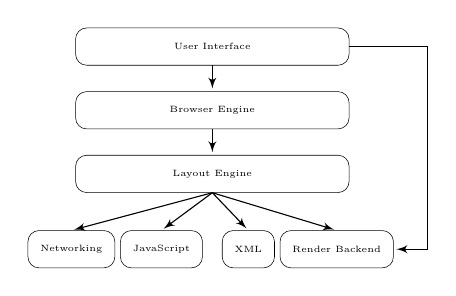
\begin{tikzpicture}[node distance=1cm, auto, transform shape, scale=0.66]  
        \tiny
          \tikzset{
              mynode/.style={rectangle,rounded corners,draw=black, top color=white, bottom color=white,very thin, inner sep=1em, minimum size=3em, text centered},
              myarrow/.style={->, >=latex', shorten >=1pt, thin},
              mylabel/.style={text width=3em, text centered}
          }  
          \node[mynode, text width=20em] (ui) {User Interface};  
          \node[mynode, text width=20em, below=0.5cm of ui] (browser-engine) {Browser Engine};
          \node[mynode, text width=20em, below=0.5cm of browser-engine] (layout-engine) {Layout Engine};
          \node[below=of layout-engine] (dummy) {};
          \node[mynode, below=of layout-engine, left=0.1cm of dummy] (javascript) {JavaScript};
          \node[mynode, below=of layout-engine, left=0.1cm and 0.1cm of javascript] (networking) {Networking};  
          \node[mynode, below=of layout-engine, right=0.1cm of dummy] (xml) {XML};
          \node[mynode, below=of layout-engine, right=0.1cm and 0.1cm of xml] (render-backend) {Render Backend};

          \draw[myarrow] (ui.south) -- (browser-engine.north);
          \draw[myarrow] (browser-engine.south) -- (layout-engine.north);
          \draw[myarrow] (layout-engine.south) -- (networking.north); 
          \draw[myarrow] (layout-engine.south) -- (javascript.north);
          \draw[myarrow] (layout-engine.south) -- (xml.north);
          \draw[myarrow] (layout-engine.south) -- (render-backend.north);
          \draw[myarrow] (ui.east) -- +(1.5, 0) |- (render-backend.east);
        \end{tikzpicture} 
        \medskip
        \caption{Reference browser architecture. The data persistance system used by the browser engine and the user interface has been omitted.} 
        \label{fig:browser_architecture}
      \end{figure}
      It is shown that the layout engine is located between the \emph{browser engine} system and the network, JavaScript, \textsc{xml} parsing and display backend.
      The browser engine acts as a high level interface to the layout engine, and is responsible for providing the layout engine with \textsc{uri}'s that should be rendered with layout options.
      The main responsibility of the layout engine is to render the current state of the fetched hypertext document.
      Since documents may (and often do) change dynamically after parse time, it is important to keep in mind that the job of the layout engine is continuous, and is not a one time operation.
      The parsing of \textsc{html} is also done by the layout engine (and not in the \textsc{xml} subsystem) since \textsc{html} is less strict and reentrant.
      In short, layout engines perform four distinct tasks:
      \begin{enumerate}
        \item Fetch of content (typically \textsc{html} and \textsc{css}) and parse it in order to construct a \textsc{dom} tree.
        \item Construct a \emph{render tree} of the \textsc{dom} tree.
        \item Layout the elements of the render tree.
        \item Render the elements of the render tree.
      \end{enumerate}
      See section~\ref{sec:dom-tree} and section~\ref{sec:render-tree} for a more in depth explanation of \textsc{dom} and render trees.
      Modern browsers can display multiple pages at the same time (by using tabs or multiple windows) where each page typically has an instance of the layout engine in a separate process.
      There are four layout engines that the major browsers use, as presented in table~\ref{table:layout_engines}.
      Since Blink is a recent fork of WebKit they can be grouped as WebKit-based layout engines.
      This results in three different layout engines to consider; WebKit, Gecko and Trident.
      Due to Trident being closed source, only the WebKit based layout engines and Gecko will be considered from now on.

      \begin{table}[ht]\center
        \tiny
        \begin{minipage}[t]{0.38\linewidth}
          \begin{tabular}[t]{ l l l }
            \textbf{Engine} & \textbf{Browsers} & \textbf{Share} \\
            \hline
            Blink & Chrome, Opera & 44.38\% \\
            WebKit & Safari & 17.64\% \\
            Trident & Internet Explorer & 14.96\% \\
            Gecko & Firefox & 12.83\% \\
          \end{tabular}
        \end{minipage}
        \hspace{0.1cm}
        \begin{minipage}[t]{0.42\linewidth}
          \begin{tabular}[t]{ l l l }
            \textbf{Engine} & \textbf{Browsers} & \textbf{Share} \\
            \hline
            WebKit & Safari, Chrome, Opera & 62.02\% \\
            Trident & Internet Explorer & 14.96\% \\
            Gecko & Firefox & 12.83\% \\
          \end{tabular}
        \end{minipage}
        \caption{
          The major layout engines and their browsers with market shares.
          The table to the right has grouped together Blink into WebKit since it is a recent for of WebKit.
          See section~\ref{sec:layout_engines_market_share} for more information how the market share data was gathered.}
        \label{table:layout_engines}
      \end{table}

      %The content fetching and parsing is an advanced topic by itself, but is not relevant for element queries since they impose no fundamental changes to process.
      %Also, rendering the final layout with the render backend is not affected by element queries.
      %The construction of 

      \section{Constructing \textsc{DOM} trees}\label{sec:dom-tree}
        \begin{metatext}
          Here a brief explanation of \textsc{dom} trees will be given, and how they are constructed.
          In order to construct a \textsc{dom} tree, the content need to be parsed which also will be covered.
          Since parsing of content is not very relevant for element queries, it will be adressed only briefly.
          This section is mainly based on \normalfont{\cite{w3c_dom}\cite{garsiel2011browsers}\cite{w3c_css21}}.
        \end{metatext}

        \textsc{dom} is an abbreviation of Document Object Model which is a convention for representing and interacting with object in \textsc{xml}-based documens (such as \textsc{html}).
        The \textsc{dom} provides an interface for programs (JavaScript scripts in the browser) to dynamically access and mutate the content, structure and style of documents.
        Each node of the document is a \textsc{dom} object, and therefore the whole document is converted to a tree structure of \textsc{dom} nodes which is refered to as the \textsc{dom} tree.

        Layout engines construct \textsc{dom} trees by parsing \textsc{html} with any included \textsc{css} and JavaScript.
        Parsing of \textsc{html} is not an easy task because the specification of \textsc{html} states that it must be forgiving (i.e. accepting malformated markup).
        \todo{Is it true that the sepc says that malformated html must be accepted. Servo experience report seems to say otherwise.}
        As \textsc{css} and JavasScript are more strict, their grammar can be expressed in a formal syntax and can therefore be parsed with a context free grammar parser (which can be autogenerated).
        Another big quirk to parsing \textsc{html} is that it is reentrant, which means that the source may change during parsing.
        Script elements are to be executed synchronously when it is occured by the parser.
        If such script mutate the \textsc{dom}, then the parser will need to evaluate the changes made by the script and update the \textsc{dom} tree.
        External scripts need to be fetched in order to be executed, which halts the parsing unless the script element states otherwise.
        It should be noted that although \textsc{dom} nodes do include a \code{style} property, the nodes in the \textsc{dom} tree are not affected by the \textsc{css} cascading, and the style properties do not represent the final style of the element.
        Instead, for scripts to obtain the final computed style for an element a special function needs to be called (\code{getComputedStyle} in JavaScript).
        Since externally linked \textsc{css} documents do not directly affect the \textsc{dom} tree they could conceptually be fetched and parsed after the parsing of the \textsc{html}.
        However, scripts can request the computed style of \textsc{dom} tree nodes and therefore either the parsing of \textsc{html} needs to be halted in order to fetch and parse \textsc{css} when it occurs, or the scripts accessing style properties of \textsc{dom} nodes need to be halted.
        A common optimization is to use a specalutive parser that continues to parse the \textsc{html} when the main parser has halted (for executing the scripts usually).
        The speculative parser does not change the \textsc{dom} tree, instead it searches for external resources that can be fetched in parallel while waiting for the main parser to continue.

        \todo{code example of reentrant html?}
        \todo{Figure of how the DOM tree looks like? Maybe example HTML and DOM tree figure.}
        \todo{Write about media type, and how the CSS is calculated if it is in this stage?}

      \section{Render trees}\label{sec:render-tree}
        \begin{metatext}
          When the \textsc{dom} tree has been constructed and all external \textsc{css} has been fetched and parsed, it is time for the layout engine to create the render tree.
          Here an explanation of the creation process and the structure of render trees will be given.
          This section is mainly based on \normalfont{\cite{garsiel2011browsers}\cite{w3c_css21}}.
        \end{metatext}

        A Render tree is a visual representation of the document.
        In contrast to the \textsc{dom} tree, the render tree only contains of elements that will be rendered.
        The nodes of the render tree are called \emph{renderers} (also known as \emph{frames} or \emph{render objects}), as the elements are responsible for laying out and rendering themselves and all of its subnodes.
        In order to know how to render themselves, the final style of each renderer needs to be computed which is done by the layout engine while constructing the tree.
        Each renderer represents a rectangle (given by style size and position) with a given style.
        There are differnt types of renderers, which affects how the renderer rectangle is computed.
        The type can be directly affected by the display style property.

        Typically nodes in the \textsc{dom} tree map in a 1:1 relation to nodes in the render tree, but the relation can also be smallar or larger.
        The render tree only contains nodes that will affect the rendered result, so nodes that do not affect the layout flow of the document and that aren't visible will not be present in the render tree.
        For instance, an \textsc{dom} node element with the \code{display} property set to \code{none} will have the relation 1:0 (it will not be present in the render tree because it is not visible and will not affect the layout flow).
        It should be noted that elements with the \code{visibility} property set to \code{hidden} will be present in the render tree, although they are not visible, since they still affect the layout flow.

        Even though all style properties have been resolved for each node in the render tree (through \textsc{css} cascading), the renderers still do not know about the size and position of the rectangle.
        This is because some properties cannot be computed by just computing the styles for an element.
        Some properties depend on the flow of the document, and needs to be resolved through a layout.
        The layout process will resolve the final position and size for all renderes.

      \section{Style computation}\label{sec:style-computation}
        \begin{metatext}
          Both the render tree and scripts need to be able to get the final style of an element.
          In order to know the final style of an element, the style for each element must be computed.
          Here a brief explanation of selector matching, style cascading, inheritence and rule set specificity will be given.
          \textsc{css} property definitions will also be described.
          This section is mainly based on \normalfont{\cite{garsiel2011browsers}\cite{w3c_css21}\cite{world2013css}}.
        \end{metatext}

        To trace how the style of an element was computed can be a complex task, since there are many parameters to element style computations.
        First, styles for an element can be defined in several places:
        \begin{enumerate}
          \item In the default styles of the browser.
          \item In the user defined browser style.
          \item In external \textsc{css} documents.
          \item In internal \textsc{css} \code{style} tags in the document head.
          \item In inline \textsc{css} in the \code{style} element attribute.
          \item In scripts modifying the element style through the \textsc{dom} tree.
          \item In special attributes of the element such as \code{bgcolor} (deprecated, but possible).
        \end{enumerate}
        This can be grouped into author, user and browser styles.
        The four first items can be regarded as \textsc{css} which means that they are \emph{cascading} their style rules through \emph{selector matching}.
        Selector matching conceptually finds all elements in the \textsc{dom} tree that matches a \textsc{css} selector, to apply the rule set.
        The rule sets are weightened so that if a property is assigned values by multiple rule sets the one with highest weight will be applied.
        The weightening process starts with the origin of the style:
        \begin{itemize}
          \item In case of normal rule declarations, the style weightening relation is: $browser < user < author$.
          \item Important rule declarations have the following relation: $author < user$.
        \end{itemize}
        The weightening process continues by calculating the \emph{specificity} of all rule set selectors, the higher the specificity the higher the rule set will be weightened.
        This will make rule sets with more specific selectors override rule sets with more general selectors.
        Finally, if two rule declarations have the same weight, origin and specificity the rule set specified last will win.
        Inline \textsc{css} does not cascade since all rules given are automatically matched with the element of the style attribute.
        However, inline \textsc{css} is considered with highest possible specificity when performing the style cascade.
        It is important to note that the styling methods number five and six are conceptually the same, since they both alter the style property of the \textsc{dom} element.
        The last item is deprecated, and all styles applied this way will be weightened as low as possible.

        If the cascade results in no value for an element style property, then the property can \emph{inherit} a value or have the initial value defined by the \textsc{css} \emph{property definition}.
        Property definitions describe how the style properties should behave, see table~\ref{table:css_property_definition}.
        For instance, the width property definition states that legal values are absolute lengths, percentages or \code{auto} (which will let the browser decide).
        The percentages are relative to the containing block.
        The initial value is \code{auto}, the properties applies to all elements non-replaced inline elements, table rows and row groups.
        The value may not be inherited, and the media groups is \code{visual}.
        The computed value is either the absolute length, calculated percentage of the containing block or what the browser decides (in case of \code{auto}).
        If a property may inherit values, it will inherit the value of the first ancestor that has a value that is not \code{inherit}.

        \begin{table}[ht]\center
          \tiny
          \begin{tabular}[t]{ r | l }
            \textbf{Value} & Defines the legal values and the syntax. \\
            \textbf{Initial} & The initial value that the property will have. \\
            \textbf{Applies to} & The elements that the property applies to. \\
            \textbf{Inherited} & Determines if the value should be inherited or not. \\
            \textbf{Percentages} & Defines if percentages are applicable, and how they should be interpreted. \\
            \textbf{Media} & Defines which media group the property applies to. \\
            \textbf{Computed value} & Describes how the value should be computed. \\
          \end{tabular}
          \caption{The \textsc{css} property definition format that describes how all element style properties behave.}
          \label{table:css_property_definition}
        \end{table}

        This process will resolve most style properties, but as stated in section~\ref{sec:render-tree} some properties require a layout in order to be resolved.

        \todo{How does selector matching work? Parallel?}
        \todo{Cascading, parallel?}

      \section{The layout process}\label{sec:layout-process}
        \begin{metatext}
          When the render tree has been constructed and the style properties has been resolved for all nodes, it is time to perform the actual layouting.
          The layout process will decide the final computed style of all elements, and needs to be done before rendering.
          This section will describe the layout process, discuss some performance aspects and show examples when layouting happens.
          This section is mainly based on \normalfont{\cite{garsiel2011browsers}}.
        \end{metatext}

        The layout (also called \emph{reflow}) of \textsc{html} is flow based which means that document layout can generally be performed top to bottom and left to right in one pass.
        This is possible because the geometry of elements typically do not depend on the siblings or children\todo{Seems weird to say that flow is not dependant on children, since the height is propagated upwards.}.
        Layout is performed recursively by starting at the root of the tree, let the renderer render itself and all of its children which will render themselves and their children and so on.
        When a layout is performed on the whole render tree it is called a \emph{global layout}.
        To avoid global layouts when an renderer has been changed, a dirty bit system is usually implemented.
        The system will mark which renderers in the tree that need a layout, which avoids layouting unaffected elements.
        Layouts that only layout the dirty renderers are called \emph{incremental layouts}.
        Layout engines that uses the dirty bit system usually keeps a queue of incremental layout commands.
        The scheduler system later triggers a batch execution of the incremental layout commands asynchronously.
        A global layout is triggered when the viewport is resized or when styles that affect the whole document are changed (such as \code{font-size}).
        Because the \textsc{api} of \code{getComputedStyle} promises resolved values for all style properties, a call will force a full layout (flushing the incremental layout commands queue).
        When a renderer performs a layout the following usually happens:
        \begin{enumerate}
          \item The own width is determined.
          \item Positions all children and request them to layout themselves (with given position and width).
          \item The heights, margins and paddings of the children are accumulated in order to decide the own height.
        \end{enumerate}
        Of course, only the children that needs a layout will be affected (dirty, or global layout) in step 2.
        So, the widths and positions are sent down in the tree and the height is sent up in the tree in order to construct the final layout.

        The widths are calculated by the \code{width} style of the elements, relative to the container element width.
        Margins and paddings are also takin into account when calculating the widths.
        When the width of an element is calculated, it needs to controlled against the \code{min-width} and \code{max-width} style properties and make sure that the width is inside the range.
        If the content of an element does not fit with the calculated width (text usually needs to perform line break when the width is too small), the element needs to break up the content into multiple renderers in order to expand the height.
        The renderer that has decided it needs to break the content up into multiple renderers propagates to the parent renderer that it needs to perform the breaking.
        When the parent renderer has created the renderes needed to fit the content with the given height, layout is performed on the new renderers and then the final height can be calculated and propageted upwards.

        \todo{Is incremental layout commands really batch processed?}

      \section{Parallelization}\label{sec:parallel}
        \begin{metatext}
          No longer can performance of an application increase over time without any code changes (as opposed to the times when \textsc{cpu} clock speeds increased rapidly).
          Now, applications need to utilize the multiple cores of the \textsc{cpu} instead of relying on high clock speed.
          Parallelization is something layout engine vendors are very interested in, and much research is being done about utilizing multiple cores to increase the speed of the engine.
          In this section a small summary will be given about the current research front, and how the parallelization can be approached.
          This section is mainly based on \normalfont{\cite{zoomm}\cite{parallelizing_the_web_browser}\cite{meyerovich2010fast}\cite{servo_parallel}\cite{servo_blog}}.
        \end{metatext}

        As web applications grow bigger and more demanding, browsers continously need to improve the performance on all levels.
        Fetching resources over the network is the only thing that is done in parallel today.
        The rest of the browser system is designed and optimized to run sequentially.
        On computers, browsers usually achieves parallelism by running each page context in parallel (each tab of the browser window is an own process).
        This approach is appealing because it utilizes the cores of the machine by still having all subsystems run sequentally for each page, while improving the overall performance of the browser.
        However, this approach is not enough.
        The page performance is not improved if only one page is present.
        For the web to be a true competitor to heavy native applications, the page performance needs to be increased (not only the overall browser performance).
        It is then important to be able to dedicate multiple cores to one page instead of having all the pages present using their own core (perhaps the non-visible pages in different tabs will share one core while the main visible tab will get access to multiple cores if needed).
        Also, with the number of mobile devices browsing the web increasing rapidly it is really important to be able to achieve good parallelism.
        Light devices such as small laptops, mobile devices and tablets share a common goal --- they want to reduce power consumption while increasing the performance.
        This can be achieved with multicore processors that run at lower clock speeds.
        \todo{Write that many cores is preferred over high clock speed? Why?}
        It has been shown that the performance of mobile browsers are \textsc{cpu} bound contrary to the common belief that they are network bandwidth bound \cite{parallelizing_the_web_browser}.
        This is why most researchers target light devices when trying to parallelize web browsers.
        Of course, once the methods has matured and been implemented, desktops will benefit from this as well.

        \textsc{css} selector matching is a good candidate for parallelization, due to matching nodes to selectors being independent from other selector matches.
        A successful parallelization of selector matching has been achieved with locality-aware task parallelism \cite{parallelizing_the_web_browser}.
        It has also been shown that selector matching and style resolving (through cascading) can be parallelized \cite{zoomm}.
        It is possible to resolve element styles in parallel as long as two requirements are fulfilled: The matching task must have finished for the element to resolve styles for, and the parent element must have resolved all styles (since the element might inherit some styles from the parent).
        As long as these requirements are fulfilled, selector matching and style resolving can run in parallel for different elements.
        The layout process can also be parallelized, since the layout process has been shown to be sub-tree independent for non-float elements \cite{servo_parallel}\cite{servo_blog}.
        Siblings of the layout tree can be processed independently of each other (in the general case), and is suitable to parallelize with a work stealing system.
        \todo{Write about the fork-join model of the parallelization as described in servo?}

    \chapter{Element queries}
      \begin{metatext}
        Now that a good understanding of browsers (especially the layout engine), responsive design and modular development has been aqcuired it is time to address element queries --- the solution to modular responsive web design.
        This chapter will define element queries, present how they solve the problem, and address some of the issues hindering element queries from being implemented natively.
        Further, some possible restrictions will be presented to resolve some of the issues.
        \todo{Instead write that some solutions will be presented?}
      \end{metatext}

      Recall from section~\ref{sec:rwd} that responsive web design is the concept of having elements respond to the given size.
      Responsive web design implements this by using media queries, applying conditional rules by the viewport size.
      In section~\ref{sec:modularity} the desire for building modular web components was presented.
      One implication of building applications in a modular way, is that general components become reusable.
      Since the only way of applying conditional rules to elements today is by using media queries, all responsive styles must be defined by the application and not by the modules (because only the application knows how much space each module will be given in the layout).
      The implication of this is that the \textsc{html} and JavaScript can be written in a modular way, but the \textsc{css} is left for the user of the module (application) to write which somewhat defeats the purpose of writing modules.
      So developers today have two choices: Writing modules that are not responsive but self contained, or writing modules that are responsive but not self contained (leaving the styling to the user).
      The solutions to this is elemenet queries, which allows conditional rules to be applied based on any criteria for any element.
      Figure~\ref{fig:mq-vs-eq} shows the problem with media queries and the element query solution.
      The typical use case is to write conditional styles to be applied based on the container element size.
      Although the typically the size of the container element is the most interesting element query with reponsive web design, element queries as a concept does not need to be limited to that.
      It is also possible to apply conditional rules by any element display property, color, text alignment, and so on.
      Theoretically it should be possible to query any style property of an element, but the focus will lay on the \code{width} and \code{height} properties since they are the most interesting in responsive web design.

      \begin{figure}
        \centering
        \begin{minipage}{.5\textwidth}
          \centering
          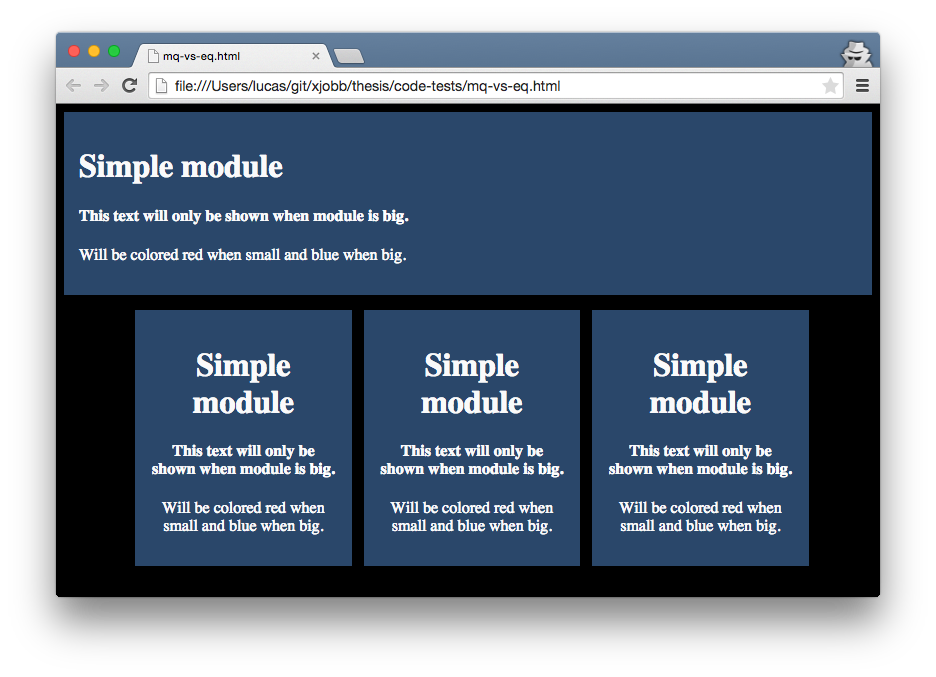
\includegraphics[width=\linewidth]{images/mq-big}
        \end{minipage}%
        \begin{minipage}{.5\textwidth}
          \centering
          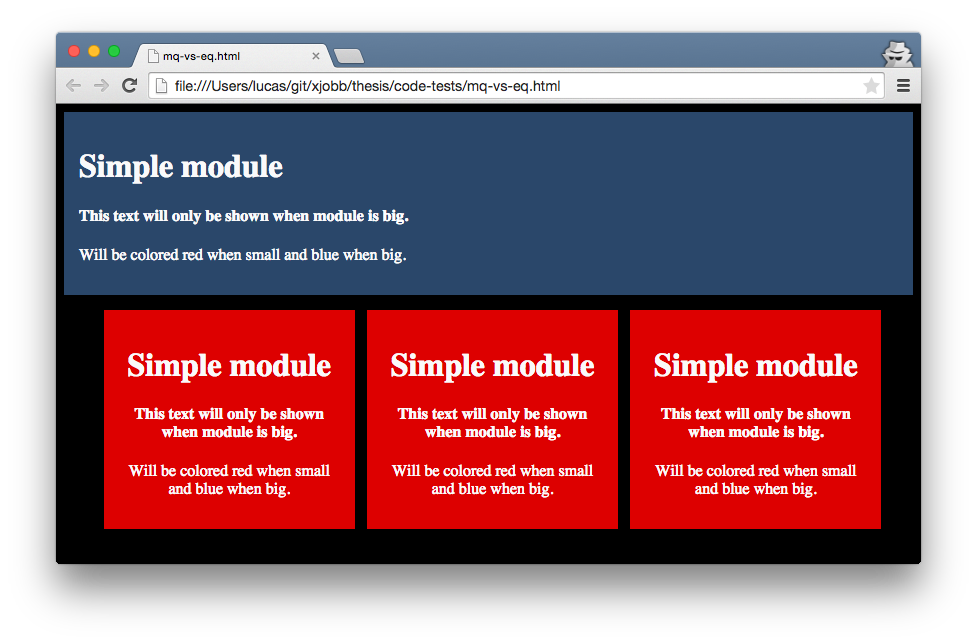
\includegraphics[width=\linewidth]{images/eq-big}
        \end{minipage}
        \caption{
          The problem of media queries and the element query solution.
          Both images shows four instances of a module in different sizes.
          The module is responsive, so when it is small it should change color to red and change the inner text a bit.
          The left version is built with media queries, hence all module instances stay blue even though some are small (only a smaller viewport will trigger the modules to change style).
          The right version is built with element queries, hence the modules display differently depending on the given size that each module has, which is the desired behavior.}
        \label{fig:mq-vs-eq}
      \end{figure}

      \section{Problems}
        \begin{metatext}
          The main reason why element queries has not been implemented natively in browsers is because they bring problems and limitations to the browsers.
          It is important to understand the problems in order to speculate about a potential native \textsc{api} design.
          In this section the two major problems will be presented; performance and circularity.
        \end{metatext}

        \todo{What to write here?}
        \subsection{Performance}
          \begin{metatext}
            This subsection will present the performance impacts that element queries have on layout engines.
            As shown in section~\ref{sec:parallel} browser vendors are very interested in parallelizing their browsers and especially the layout engines to increase the page performance.
            Element queries limits the parallelization badly, which will be the focus of this subsection.
            \todo{Referera till w3c mailinglista?}
          \end{metatext}

          Recall from section~\ref{sec:layout-process} that the box size and position for each element is calculated at in the layout process, and cannot be determined before an actual layout has happened.
          This impose that a layout pass needs to be performed before knowing the element sizes.
          If element queries are present that rely on the size of elements, which is the identified common usecase, the following process needs to happen:
          \begin{enumerate}
            \item A layout pass needs to be performed in order to calculate the size of the elements targeted by element queries.
            \item The element query conditional rules need to be evaluated against the elements to know which rules should be applied (element query selector matching).
            \item If the element query selector matching has resulted in a different matching set than in step 1, another layout pass (with the new rules applied) needs to be performed.
          \end{enumerate}
          So for each element query selector matching change result in performing another layout, discarding at least a subtree of the previous layout.
          As already stated, this only occurs when the layout has changed in a way that changes the element query selectors.
          Unfortunately, this means that if there is any matching element query selector at page load, two layout passes will always be performed.

          Further, it is common for internal \textsc{api}'s in layout engines to request updated element styles that do not require layout to resolve (non-layout properties such as \code{color} and \code{font-family}).
          Since a layout of the element query selector target is required in order to resolve the correct element style, such internal \textsc{api}'s will require a layout in order to obtain the correct element style (even for non-layout related properties).
          Also, layout engines would not be able to layout subtrees in parallel since an element in one subtree might affect an element in another subtree.

          \todo{Totally forgot to write about parallel problems}

        \subsection{Circularity}\label{sec:cyclic-rules}
          \begin{metatext}
            This subsection will show how cyclic rules may occur and why it is such a major problem.
            It will also be presented why cyclic rules must be detected at run time.
            Some examples of will be given to better understand the complexity of the problem.
          \end{metatext}

          The most straight forward occurances of cyclic rules are when there are specified conflicting width constraints and width updates for an element.
          See listing~\ref{code:cyclic-simple} for the perhaps most simple example of cyclic rules.
          The syntax of element queries will be presented in section~\ref{}, and is not important to understand the problem.
          \begin{lstlisting}[caption={Very simple example of cyclic rules.}, captionpos=b, label={code:cyclic-simple}]
#foo {
  width: 250px;
}

#foo:eq(max-width: 300px) {
  /* This rule will be applied only when the width of #foo is < 300px. */
  width: 550px;
}

#foo:eq(min-width: 500px) {
  /* This rule will be applied only when the width of #foo is > 500px. */
  width: 250px;
}
          \end{lstlisting}

          The following will happen to the element:
          \begin{enumerate}
          \item The initial width of the \code{\#foo} element is set to 250 pixels.
          After a layout, the \code{\#foo:eq(max-width: 300px)} will match and therefore next step will be 2.
          \item The width of the element is under 300 pixels, so the selector \code{\#foo:eq(max-width: 300px)} will match.
          Note that the \code{\#foo:eq(min-width: 500px)} does not match, since the width is under 500 pixels.
          Since the matched selector is more specific than the \code{\#foo} selector, the new width of the element will be 550 pixels.
          Next step will be 3.
          \item The width of the element is above 500 pixels, so the selector \code{\#foo:eq(min-width: 500px)} will match.
          Note that the \code{\#foo:eq(max-width: 300px)} does not match, since the width is above 300 pixels.
          Since the matched selector is more specific than the \code{\#foo} selector, the new width of the element will be 250 pixels.
          Next step will be 2.
          \end{enumerate}
          Clearly, the browser will be stuck in an infinite layout cycle pending back and forth between step 2 and 3 (250 pixels and 550 pixels).
          The result of this is of course implementation dependant.
          One reasonable outcome of such infinite layout loop is that the layout engine will execute one layout pass and then evaluate the next set of matched selectors and so on, which will lead to a functioning site but since a relayout is enforced every update, the performance impact will be huge.
          This example is somewhat similar to writing \code{while(true);} in JavaScript, which obviously is a bad idea.
          However, cyclic rules can also occur in less obvious ways. 

          Indirect cyclic rules are somewhat more complex to reason about, than the example given above (which is an example of direct cyclic rules).
          For instance, if the \code{\#foo} element matches the width of a child element, and the child changes width depending on the parent width, a cycle might occur.
          Consider the code in listing~\ref{code:cyclic-2}.
          
          \begin{lstlisting}[caption={Example of indirect cyclic rules.}, captionpos=b, label={code:cyclic-2}]
/* HTML */
<div id="foo">
  <div id="child"></div>
</div>

/* CSS */
#foo {
  /* Will match the width of the child element. */
  display: inline-block;
}

#child {
  width: 250px;
}

#foo:eq(max-width: 300px) #child {
  /* This rule will be applied only when the width of #foo is < 300px. */
  width: 550px;
}

#foo:eq(min-width: 500px) #child {
  /* This rule will be applied only when the width of #foo is > 500px. */
  width: 250px;
}
          \end{lstlisting}
          What makes this situation more complex than the previous example is that it is less obvious for numerous reasons:
          \begin{itemize}
            \item The rules of the child element and the rules of the \code{\#foo} element might be separated into different parts of the stylesheet (or even different stylesheets).
            The problem cannot be found without considering both of the rule sets.
            \item The child element might be another module, and by adding one line to the parent module (the \code{\#foo} element) a cycle has appeared.
            \item The developer has to be well aware of how the display property affects the element and what implications the \code{inline-block} has to the element.
          \end{itemize}
          An JavaScript quivalent of this example would perhaps be \code{var bar = true; while(bar);} with the motivation that it is still very obvious that it is an infinite loop but both the while loop and the variable needs to be reviewed.
          Also, the variable assignment could happen in another part of the program.

          The examples given so far have been simple and easily detectable.
          However, cycles can occur in a much more complex way.
          The two given examples could both be identified as cyclic by simply reviewing the \textsc{css} code.
          It is also possible for a program to analyze the examples to deduce that they are cyclic.
          Unfortunately, not all cycles can be detected by static analyze.
          Consider the code in listing~\ref{code:cyclic-3}.
          \begin{lstlisting}[caption={Example of indirect cyclic rules.}, captionpos=b, label={code:cyclic-3}]
/* HTML */
<div id="foo">
  <div id="child">
    When in doubt, mumble.
  </div>
</div>

/* CSS */
#foo {
  /* Will match the width of the child element. */
  display: inline-block;
}

#child {
  font-size: 1.5em;
}

#foo:eq(max-width: 300px) #child {
  /* This rule will be applied only when the width of #foo is < 300px. */
  font-size: 3em;
}

#foo:eq(min-width: 500px) #child { 
  /* This rule will be applied only when the width of #foo is > 500px. */
  font-size: 1em;
}
          \end{lstlisting}
          In this example, it is virtually impossible to tell if the rules are cyclic.
          So what happens is that the \code{\#foo} element will get the size of the child element, which width depend on the text inside it.
          The width of the text depends on the font size, which is initially set to \code{1.5em}.
          The \code{em} unit is relative to the inherited font size of the element.
          So the width of the \code{\#foo} element is dependent on the inherited font size.
          When the \code{\#foo} element is below 300 pixels wide, the font size of the child is increased to \code{3em} and when above 500 pixels the font size is decreased to \code{1em}.
          So if \code{3em} results in a font size big enough to make the child element bigger than 500 pixels, and if \code{1em} results in a font size small enough to make the child element smaller than 300 pixels the rules are cyclic.
          The factors that creates the cycle are the following:
          \begin{itemize}
            \item The display type of the \code{\#foo} element
            \item The element queries of the child element
            \item The font size value of the child element
            \item \textbf{The inherited font size of the \code{\#foo} element}
            \item \textbf{The text of the child element}
          \end{itemize}
          The bolded factors are of a far worse type than the ones presented until now.
          They are impossible to determine at parse time.
          In this example the text is static but it could have beeen added dynamically.
          Also, the inherited font size depends on the closest ancestor with a font size property defined.
          Since ancestors also can have their font sizes defined in relative units, the dependency tree can go up to the root of the document.
          Further, if no ancestor defines an absolute value for the font size it is up to the browser to default to a size, which is impossible to reason about at parse time.
          This implies that there is no way of telling if the cycle will appear or not without actually running the code.
          Also, the cycle may appear in different browsers and settings, which makes the cycle even harder to detect.
          Far worse is that the previous examples have been of the \code{while(true);} character, which gives the false hope that even though it is possible to create cycles developers would never encouter it since ``real'' code would not be close to the examples given here.
          With the third example, this is no longer true.
          Increasing the font size when the layout area is smaller and decreasing the font size when the layout area is bigger is something that is frequently done in responsive web deisgn.
          Typically web site authors want the font size to increase on handheld devices, to increase the readability.
          Of course, the numbers given in the example might not be reasonable, but in concept it is valid use case which may result in cyclic rules.

      \section{Possible solutions}
        \begin{metatext}
          Now that the problems of element queries have been presented, it is time to show some possible solutions to the problems.
          The different solution approaches either limits element queries in some way or solves only a subproblem, so no perfect solution that keeps element queries unlimited with decent performance has been found.
        \end{metatext}

        \todo{Write somewhere that iframes are not a solution? But they are close to a solution...}
        \subsection{Viewport elements}
          \begin{metatext}
            This solution limits element queries a lot, but avoids many of the problems this way.
            This approach has been discussed at \textsc{w3c} and \textsc{ricg} assumes that this is a prerequisite to a native implementation.
            \todo{cite where this has been gathered from?}
          \end{metatext}

          By limiting element queries to special \emph{viewport} container elements that can only be queried by child elements, much of the problems are resolved.
          This means that a new \textsc{html} tag will be crafted (perhaps named \code{viewport}) that defines separated viewports in the document.
          The size of Viewports are not dependent on their children, and children may only target the closest ancestor viewport element in the element queries.
          This way, cyclic rules can no longer occur since the viewport size may not be altered by the children.

          This approach also solves many of the performance problems, but not all.
          The internal \textsc{api}'s that request non-layout information for the elements using element queries only need to make sure that the containging viewport element has been layed out before resolving the styles (which is a much better situation that the unrestricted version of element queries).
          Further, the layout can be done in one pass as long as the viewport elements are layed out before the children.
          It is still a bit inconvenient that the layout engine would need to evaluate all element query selectors in the middle of a layout pass (after the that the viewport elements has been layed out) in orde to resolve the styles for the viewport children.
          Parallelization is also easier, since the queries may only be targeting the closest viewport element.
          This means that each viewport subtree can be layed out in parallel.

          This solution would behave much like the \code{iframe} element layout-wise.
          It should be noted that \code{iframe} elements are not suitable as an alternative to the proposed \code{viewport} elements, since \code{iframe}'s are much more limited by nature (creates a new document and script context).

          Obviously, this limits element queries a lot.
          The fact that the size of the viewport element cannot depend on the children (like normal block elements do), limits the usability.
          The idea is that the viewport cannot cannot be queried for properties that the children may affect (such as the width and height style properties).
          In order to allow the children to query the properties, they cannot be affected by the children.
          In theory it should mean that if no children query for instance the height of the viewport, then the viewport may depend on the children for it's height.
          This is a powerful insight, since the general use case would be to write element queries against the width and have the elements adapt their heights accordingly (including the viewport element).
          \todo{Back this up. Maybe check with RICG if this is possible?}

        \subsection{Element queries with runtime checks}
          \begin{metatext}
            This solution does not limit element queries, but does also not solve all problems.
            Instead of making cyclic rules impossible, a mechanism to handle the cyclic rules is desired.
            Unfortunately this does not improve the performance at all, which is a major drawback.
          \end{metatext}

          \todo{Should this be incorporated with some other section or be written?}
          \todo{Maybe write about having a third-party framework as a solution?}
      \section{Native API design}
        \begin{metatext}
          In this section a possible native element query \textsc{api} will be presented.
          This is based on the current information and approaches of \textsc{w3c} and \textsc{ricg}, and should therefore be regarded as a guideline to how an \textsc{api} might look like.
        \end{metatext}


  \part{Third-party framework}
    \chapter{Analysis of approaches}
    \section{Current implementations}
    \chapter{API design}
    \chapter{Implementation}
      \section{Element resize events}
        \subsection{Native resize event}
        \subsection{Object injection}
  \part{Result}
    \chapter{Discussion}
  \printbibliography
    \appendix
    \addappheadtotoc
      \chapter{Resources}
        \section{Practical problem formulation document}\label{sec:problem-formulation}
          TODO: Should this be in the real document instead of appendix?          
        \section{CSS terminology}
          TODO: Write custom or refer to this \url{http://www.impressivewebs.com/css-terms-definitions/}?
        \section{Layout engine market share statistics}\label{sec:layout_engines_market_share}
          Browser market share was retrieved by \emph{StatCounter}\footnote{StatCounter graph \url{http://gs.statcounter.com/\#all-browser-ww-monthly-201402-201502-bar}}.
          Since the graph only display browser market share and not layout engine, it is needed to further divide the browsers into layout engine percentages.
          The Blink engine was introduced with Chrome version 28 and Android version 4.4 \cite{wiki_blink}.
          Since Chrome has very good adoption rate\footnote{According to \url{http://clicky.com/marketshare/global/web-browsers/google-chrome/}} of new versions the Chrome market share percentage of 39.72\% is considered to be Blink based.
          However, Android has not as good adoption rate as Chrome with only 44.2\% using Android version 4.4 and up\footnote{According to \url{https://developer.android.com/about/dashboards/index.html}}.
          Android has a browser market share of 7.21\%. 44.2\% of the 7.21\% Android browsers is assumed to be Blink based and 55.8\% to be WebKit based (since the Android browser was WebKit based before Blink).
          Of course, the assumption that users with old versions of Android browse the web as much as users with new versions are probably invalid, but the data source itself is uncertain enough to make such assumptions and the percentages should only be regarded as guidelines.
          Opera with the lowest market share at 3.97\% started using the Blink engine in late 2013 as of version 15.
          StatCounter shows that 37\% of the Opera users are using Opera Mini (their mobile browser), which does not use the Blink engine (it uses Opera's own Presto layout engine which will be ignored).
          All desktop users of Opera are assumed to be using version 15 or above and hence using the Blink engine.
          The total market share percentage of the Blink engine is then calculated to $39.72 + 0.442\cdot7.21 + 0.37\cdot3.97 = 44.38\%$.
          Safari, with the market share percentage of 7.46\%, has always been WebKit based.
          iOS also uses WebKit and has the market share percentage of 6.16\%.
          The WebKit market share percentage is calculated to $7.46 + 0.558\cdot7.21 + 6.16 = 17.64\%$.
          FireFox, with the market share percentage of 12.83\%, has always been Gecko based and is the only major browser that uses the Gecko engine.
          The market share percentage of Gecko is therefore 12.83\%.
          Internet Explorer, with the market share percentage of 14.96\%, has been Trident based since version 4.
          Since Internet Explorer 4 is no longer in use\footnote{According to \url{http://www.w3schools.com/browsers/browsers_explorer.asp}}, the market share percentage of the Trident engine is 14.96\%.
\end{document}
